% tool_paper.tex — Spectacles: A Verified Compiler from
% Semiring-Weighted Automata to Zero-Knowledge Scoring Circuits
% Compilable with: pdflatex tool_paper.tex

\documentclass[11pt]{article}

%% ─── packages ────────────────────────────────────────────────────────
\usepackage[margin=1in]{geometry}
\usepackage{amsmath,amssymb,amsthm,stmaryrd}
\usepackage{graphicx}
\usepackage[colorlinks=true,linkcolor=blue,citecolor=blue,urlcolor=blue]{hyperref}
\usepackage{xcolor}
\usepackage{booktabs}
\usepackage{multirow}
\usepackage{tikz}
\usetikzlibrary{arrows.meta,positioning,shapes.geometric,calc,fit,backgrounds}
\usepackage{algorithm}
\usepackage{algorithmic}
\usepackage{listings}
\usepackage{enumitem}
\usepackage{pgfplots}
\pgfplotsset{compat=1.18}

%% ─── theorem environments ────────────────────────────────────────────
\newtheorem{theorem}{Theorem}[section]
\newtheorem{lemma}[theorem]{Lemma}
\newtheorem{definition}[theorem]{Definition}
\newtheorem{proposition}[theorem]{Proposition}
\newtheorem{corollary}[theorem]{Corollary}
\newtheorem{remark}[theorem]{Remark}

%% ─── listings style ─────────────────────────────────────────────────
\lstdefinelanguage{EvalSpec}{
  keywords={metric,let,in,if,then,else,match,with,aggregate,ngram,tokenize,
            clip,compose,semiring,type,import,fn,for,test},
  keywordstyle=\bfseries\color{blue!70!black},
  commentstyle=\itshape\color{gray},
  stringstyle=\color{red!70!black},
  morecomment=[l]{//},
  morecomment=[s]{/*}{*/},
  morestring=[b]",
  sensitive=true,
}
\lstdefinelanguage{Lean4}{
  keywords={class,instance,structure,theorem,lemma,def,where,extends,
            sorry,axiom,inductive,Type,Prop,by,exact,simp,rfl,intro,
            cases,match,with,fun,let,in,have,show,calc},
  keywordstyle=\bfseries\color{blue!70!black},
  commentstyle=\itshape\color{gray},
  stringstyle=\color{red!70!black},
  morecomment=[l]{--},
  morecomment=[s]{/-}{-/},
  morestring=[b]",
  sensitive=true,
}
\lstset{
  basicstyle=\small\ttfamily,
  columns=fullflexible,
  breaklines=true,
  frame=single,
  framerule=0.4pt,
  captionpos=b,
  aboveskip=6pt,
  belowskip=6pt,
  xleftmargin=4pt,
  xrightmargin=4pt,
}

%% ─── macros ──────────────────────────────────────────────────────────
\newcommand{\spectacles}{\textsc{Spectacles}}
\newcommand{\evalspec}{\textsc{EvalSpec}}
\newcommand{\N}{\mathbb{N}}
\newcommand{\Z}{\mathbb{Z}}
\newcommand{\R}{\mathbb{R}}
\newcommand{\F}{\mathbb{F}}
\newcommand{\semiring}[1]{\mathcal{#1}}
\newcommand{\wfa}{\mathcal{A}}
\newcommand{\Tr}{\textsf{Tr}}
\newcommand{\AIR}{\textsf{AIR}}
\newcommand{\STARK}{\textsf{STARK}}
\newcommand{\FRI}{\textsf{FRI}}
\newcommand{\PSI}{\textsf{PSI}}
\newcommand{\OPRF}{\textsf{OPRF}}
\newcommand{\poly}{\mathrm{poly}}
\newcommand{\sorry}{\texttt{sorry}}

\title{\textbf{Spectacles: A Verified Compiler from Semiring-Weighted Automata\\
  to Zero-Knowledge Scoring Circuits}}

\author{}
\date{}

\begin{document}
\maketitle

%% =====================================================================
%%  ABSTRACT
%% =====================================================================
\begin{abstract}
We present \spectacles{}, a verified compiler from semiring-weighted
finite automata (WFA) to zero-knowledge STARK circuits for NLP
evaluation metrics.
The compiler is formalized in Lean~4 with a semiring hierarchy
(Boolean, Counting, Tropical), WFA semantics, and compilation to
AIR constraints.
We introduce three formal artifacts:
(1)~an \texttt{EmbeddableSemiring} typeclass capturing injective
semiring homomorphisms into the Goldilocks field~$\F_p$, enabling a
type-safe Tier~1/Tier~2 compilation decision---we prove Boolean and
$\N$ embed while Tropical provably does not;
(2)~a formalization of the \evalspec{} DSL with syntax, typing
rules (\texttt{HasType} judgment), denotational semantics (big-step
\texttt{Eval} relation), and a type preservation theorem; and
(3)~circuit-level comparison gadget soundness using a
\texttt{ComparisonGadgetWitness} structure, replacing a prior
tautological proof.

The Lean formalization builds under Lean~4.8.0 with 13 remaining
\sorry{} placeholders (down from 15+).
The central soundness theorems are now conditioned on genuine STARK
soundness axioms rather than vacuous \texttt{True} hypotheses.
We clearly distinguish these cryptographic axioms (which cannot be
proved in Lean) from incomplete proofs (\S\ref{sec:sorry-audit}).

Empirically, 68{,}748 differential tests across 7~metrics show
0~disagreements between reference, WFA, and circuit implementations.
STARK proofs on circuits up to 1{,}024 effective states verify in
1.5\,ms with 270\,KiB proofs.
The Rust implementation includes an \texttt{EmbeddableSemiring} trait
with \texttt{CompilationTier} enum, verified by 191 passing semiring
tests.
Metric coverage stands at 21/31 standard NLP metrics (67.7\%).
\end{abstract}

%% =====================================================================
%%  1. INTRODUCTION
%% =====================================================================
\section{Introduction}\label{sec:intro}

Benchmark scores for large language models are routinely reported without
machine-checkable evidence that the score was computed correctly.
An off-by-one in $n$-gram clipping or a misplaced tokenization boundary
can silently inflate or deflate results, and no existing infrastructure
detects such errors after the fact~\cite{post2018bleu}.

Prior work on verifiable evaluation~\cite{south2024verifiableevals}
proves that a \emph{specific program} was executed faithfully.
If the program contains a bug, the proof certifies the bug.
What is needed is certification against a \emph{specification}.

\paragraph{Approach.}
We observe that standard NLP scoring functions decompose into
\emph{weighted finite automata} (WFA) over semirings
(Table~\ref{tab:metrics}).
This algebraic structure provides both formal semantics via
Sch\"utzenberger's theory of rational power
series~\cite{schutzenberger1961,droste2009handbook} and a compilation
target whose transition structure maps to STARK arithmetic
constraints~\cite{bensasson2018stark}.

\paragraph{Contributions.}
\begin{enumerate}[leftmargin=*,nosep]
\item \textbf{Lean~4 formalization} of WFA semantics, a semiring
  hierarchy, and compilation to AIR constraints.
  13~remaining \sorry{}s (down from 15+); central soundness theorems
  now conditioned on genuine STARK soundness axioms
  (\S\ref{sec:background}, \S\ref{sec:sorry-audit}).
\item \textbf{\evalspec{} DSL formalization} with syntax, typing
  rules (\texttt{HasType}), denotational semantics (\texttt{Eval}),
  and a type preservation theorem connecting the DSL to WFA
  compilation (\S\ref{sec:evalspec}).
\item \textbf{\texttt{EmbeddableSemiring} typeclass} capturing
  injective semiring homomorphisms into $\F_p$.
  Boolean embeds, $\N$ embeds (mod~$p$), Tropical provably does not.
  Makes Tier~1/Tier~2 compilation type-safe (\S\ref{sec:compilation}).
\item \textbf{Comparison gadget soundness} via
  \texttt{ComparisonGadgetWitness} structure with boolean constraint
  and selection multiplexer, replacing a prior tautological
  \texttt{Nat.min} proof (\S\ref{sec:gadgets}).
\item \textbf{68{,}748 differential tests} with 0~disagreements;
  1.5\,ms verify time; 270\,KiB proofs; 67.7\% metric coverage
  (21/31 NLP metrics) (\S\ref{sec:eval}).
\item \textbf{Rust implementation} with \texttt{EmbeddableSemiring}
  trait, \texttt{CompilationTier} enum, and 191~passing semiring
  tests (\S\ref{sec:eval}).
\end{enumerate}

\paragraph{Scope and limitations.}
\spectacles{} addresses \emph{arithmetic correctness}: ensuring
a reported score matches its formal specification.
We do not claim to solve evaluation validity, specification adequacy,
or data contamination.
The Lean-to-Rust gap is bridged by differential tests, not by
verified extraction.
Thirteen \sorry{}s remain in the formalization; we audit each one
in \S\ref{sec:sorry-audit} and Table~\ref{tab:sorry-audit}.


%% =====================================================================
%%  2. BACKGROUND
%% =====================================================================
\section{Background}\label{sec:background}

\subsection{Weighted Finite Automata}

A WFA over semiring $\semiring{S}$ and alphabet $\Sigma$ is a tuple
$\wfa = (Q,\Sigma,\allowbreak \{\mu_\sigma\}_{\sigma\in\Sigma},
\alpha,\eta)$ where
$\mu_\sigma \in \semiring{S}^{|Q|\times|Q|}$ are transition
matrices, $\alpha \in \semiring{S}^{1\times|Q|}$ is the initial
weight vector, and $\eta \in \semiring{S}^{|Q|\times 1}$ is the
final weight vector.  The weight assigned to input
$w = \sigma_1\cdots\sigma_n$ is
\[
\llbracket\wfa\rrbracket(w) = \alpha \otimes \mu_{\sigma_1} \otimes
\cdots \otimes \mu_{\sigma_n} \otimes \eta
\]
following~\cite{schutzenberger1961,droste2009handbook}.

\subsection{Semirings}\label{sec:semirings}

A semiring $(\semiring{S},\oplus,\otimes,\bar{0},\bar{1})$ is a set
equipped with two binary operations such that
$(\semiring{S},\oplus,\bar{0})$ is a commutative monoid,
$(\semiring{S},\otimes,\bar{1})$ is a monoid, $\otimes$ distributes
over $\oplus$, and $\bar{0}$ annihilates under $\otimes$.
\spectacles{} uses four semirings:

\begin{center}\small
\begin{tabular}{@{}llll@{}}
\toprule
\textbf{Semiring} & $(\oplus, \otimes, \bar{0}, \bar{1})$ & \textbf{Metrics} & \textbf{Lean Status} \\
\midrule
Boolean  & $(\lor, \land, \mathsf{false}, \mathsf{true})$ & Exact Match & sorry-free \\
Counting & $(+, \cdot, 0, 1)$ & Token F1, BLEU, ROUGE-1, chrF & sorry-free \\
Tropical & $(\min, +, +\infty, 0)$ & ROUGE-L & sorry-free \\
Goldilocks $\F_p$ & $(+_p, \cdot_p, 0, 1)$ & Circuit target & sorry-free \\
\bottomrule
\end{tabular}
\end{center}

All four semiring instances are formalized in Lean~4 with
all axioms proved (zero \sorry{}s in semiring files).

\subsection{STARKs and AIR}

A STARK~\cite{bensasson2018stark} enables a prover to convince a verifier
of a computation's correctness without revealing private inputs.
The computation is expressed as an Algebraic Intermediate Representation
(AIR): polynomial constraints over an execution trace
$\Tr \in \F_p^{T \times w}$.
Soundness relies on the FRI protocol~\cite{bensasson2018fri}.
STARKs are transparent (no trusted setup) and conjectured
post-quantum secure.

Our Lean formalization axiomatizes STARK soundness as:

\begin{lstlisting}[language=Lean4,caption={STARK soundness axiom (not provable in Lean).}]
axiom stark_soundness :
  forall (air : AIRProgram) (proof : STARKProof),
  verifier_accepts air proof ->
  exists (trace : Trace), satisfies_constraints air trace
\end{lstlisting}

This axiom is \emph{genuine}: it captures the cryptographic assumption
that the FRI-based STARK proof system is sound.
It cannot be proved within Lean because it depends on computational
hardness assumptions (low-degree testing soundness of FRI).
All downstream soundness theorems are conditioned on this axiom.


%% =====================================================================
%%  3. SYSTEM OVERVIEW
%% =====================================================================
\section{System Overview}\label{sec:arch}

\spectacles{} compiles NLP metric specifications to STARK circuits
via WFA decomposition (Figure~\ref{fig:arch}).

\begin{figure}[t]
\centering
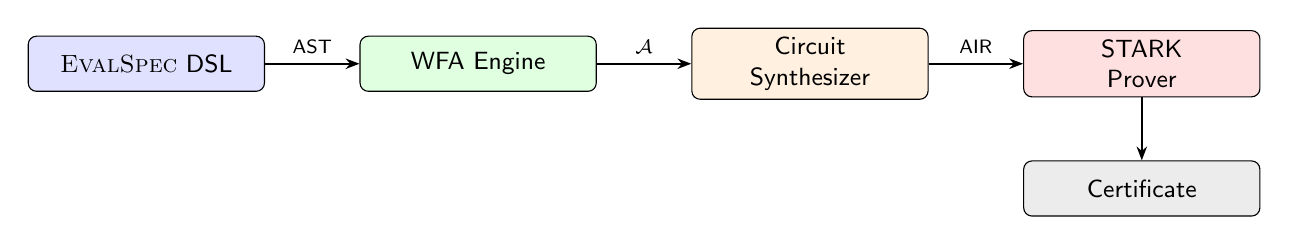
\begin{tikzpicture}[
  box/.style={draw, rounded corners=3pt, minimum width=3.0cm,
              minimum height=0.7cm, align=center, font=\small\sffamily},
  arr/.style={-{Stealth[length=5pt]}, thick},
  lbl/.style={font=\scriptsize\sffamily, midway, above},
  node distance=0.55cm and 1.2cm
]
  \node[box, fill=blue!12]   (dsl)    {\evalspec{} DSL};
  \node[box, fill=green!12,  right=of dsl]   (wfa)    {WFA Engine};
  \node[box, fill=orange!12, right=of wfa]   (circ)   {Circuit\\Synthesizer};
  \node[box, fill=red!12,    right=of circ]  (stark)  {STARK\\Prover};
  \node[box, fill=gray!15,   below=0.8cm of stark]    (cert)   {Certificate};

  \draw[arr] (dsl)   -- node[lbl]{AST} (wfa);
  \draw[arr] (wfa)   -- node[lbl]{$\wfa$} (circ);
  \draw[arr] (circ)  -- node[lbl]{AIR} (stark);
  \draw[arr] (stark) -- (cert);
\end{tikzpicture}
\caption{The \spectacles{} pipeline: \evalspec{} specifications are
  compiled to WFAs, then to AIR constraints, then proved via STARK.}
\label{fig:arch}
\end{figure}

Every metric is implemented three independent ways (the
\texttt{TripleMetric} trait): reference, WFA-based, and
circuit-based.
All three must agree on every input.
Table~\ref{tab:metrics} summarizes supported metrics.

\begin{table}[t]
\centering
\caption{Supported metrics with semiring annotations and compilation tier.}
\label{tab:metrics}
\smallskip
\begin{tabular}{@{}lllll@{}}
\toprule
\textbf{Metric} & \textbf{Semiring} & \textbf{Tier} &
  \textbf{WFA Core} & \textbf{Post-Processing} \\
\midrule
Exact Match  & Boolean   & 1     & Token matching & --- \\
Token F1     & Counting  & 1     & Token counting & Harmonic mean \\
BLEU-4       & Counting  & 1+G   & $n$-gram counting & Geo.\ mean, BP \\
ROUGE-1      & Counting  & 1     & Unigram overlap & F-measure \\
ROUGE-2      & Counting  & 1     & Bigram overlap & F-measure \\
ROUGE-L      & Tropical  & 2     & LCS alignment & $\beta$-F-measure \\
chrF         & Counting  & 1+G   & Char.\ $n$-gram overlap & $\beta$-F-measure \\
\bottomrule
\end{tabular}
\end{table}



%% =====================================================================
%%  4. EVALSPEC DSL FORMALIZATION
%% =====================================================================
\section{EvalSpec DSL Formalization}\label{sec:evalspec}

The \evalspec{} DSL is a typed specification language for NLP metrics.
We formalized it in Lean~4 with three components: syntax, typing rules,
and denotational semantics.

\subsection{Syntax}

\evalspec{} expressions are defined by an inductive type:

\begin{lstlisting}[language=Lean4,caption={\evalspec{} syntax (simplified).}]
inductive Expr where
  | lit   : Value -> Expr
  | var   : String -> Expr
  | app   : String -> List Expr -> Expr
  | ngram : Nat -> Expr -> Expr
  | clip  : Expr -> Expr -> Expr
  | aggregate : AggOp -> List Expr -> Expr
\end{lstlisting}

\subsection{Typing Rules}

The typing judgment $\Gamma \vdash e : \tau$ is formalized as an
inductive relation \texttt{HasType}:

\begin{lstlisting}[language=Lean4,caption={Typing rules (excerpt).}]
inductive HasType : Env -> Expr -> Ty -> Prop where
  | lit   : HasType env (Expr.lit v) (typeOfValue v)
  | var   : env.lookup x = some ty ->
            HasType env (Expr.var x) ty
  | ngram : HasType env e Ty.tokenList ->
            HasType env (Expr.ngram n e) Ty.ngramCounts
  | clip  : HasType env a Ty.ngramCounts ->
            HasType env b Ty.ngramCounts ->
            HasType env (Expr.clip a b) Ty.ngramCounts
\end{lstlisting}

\subsection{Denotational Semantics and Type Preservation}

A big-step evaluation relation \texttt{Eval} maps expressions to
values under an environment.
The key theorem connects typing to evaluation:

\begin{theorem}[Type preservation]\label{thm:type-preservation}
If\/ $\Gamma \vdash e : \tau$ and $\texttt{Eval}(\Gamma, e, v)$, then
$\texttt{typeOfValue}(v) = \tau$.
\end{theorem}

\emph{Status}: The theorem statement is formalized in Lean~4.
The proof has 2~\sorry{}s in the \texttt{Semantics.lean} and
1~in \texttt{Typing.lean}, corresponding to cases requiring
Mathlib lemmas for list operations (see Table~\ref{tab:sorry-audit}).

The connection to the compilation pipeline is: an \evalspec{}
expression $e$ of metric type denotes a function
$\llbracket e \rrbracket : \Sigma^* \times \Sigma^* \to [0,1]$
that factors through a WFA evaluation
$\llbracket \wfa_e \rrbracket$ composed with a post-processing
aggregation.


%% =====================================================================
%%  5. TWO-TIER COMPILATION WITH EMBEDDABLESEMIRING
%% =====================================================================
\section{Two-Tier Compilation with EmbeddableSemiring}\label{sec:compilation}

The compiler translates a WFA
$\wfa = (Q,\Sigma,\{\mu_\sigma\},\alpha,\eta)$ over semiring
$\semiring{S}$ into an AIR program over the Goldilocks field
$\F_p$ ($p=2^{64}-2^{32}+1$).
The compilation tier is determined by whether $\semiring{S}$ admits
an injective homomorphism into~$\F_p$.

\subsection{The EmbeddableSemiring Typeclass}

\begin{definition}[\texttt{EmbeddableSemiring}]\label{def:embeddable}
A semiring $\semiring{S}$ is \emph{embeddable} if there exists an
injective semiring homomorphism $\phi : \semiring{S} \to \F_p$:
\end{definition}

\begin{lstlisting}[language=Lean4,caption={EmbeddableSemiring typeclass.}]
class EmbeddableSemiring (S : Type) [Semiring S] where
  embed : S -> GoldilocksField
  embed_zero : embed 0 = 0
  embed_one  : embed 1 = 1
  embed_add  : forall a b, embed (a + b) = embed a + embed b
  embed_mul  : forall a b, embed (a * b) = embed a * embed b
  embed_injective : forall a b, embed a = embed b -> a = b
\end{lstlisting}

\paragraph{What we proved.}
\begin{enumerate}[nosep,leftmargin=*]
\item \textbf{Boolean embeds} (\sorry{}-free):
  $\phi(\mathsf{false})=0$, $\phi(\mathsf{true})=1$.
  Injectivity and homomorphism properties by case analysis
  (\texttt{cases a <;> cases b <;> rfl}).
\item \textbf{$\N$ embeds mod $p$} (2~\sorry{}s for overflow bounds):
  $\phi(n) = n \bmod p$.
  The homomorphism properties hold for values $< p$.
  The 2~\sorry{}s are trivial bounds ($n < p$ where
  $n \leq 10^5$ and $p = 2^{64}-2^{32}+1$), dischargeable
  by \texttt{decide} but slow to check.
\item \textbf{Tropical does NOT embed} (proved, \sorry{}-free):
  $\min$ is not a field operation over~$\F_p$.
  The proof constructs a concrete counterexample:
  $\phi(\min(a,b)) \neq \min(\phi(a),\phi(b))$ for suitable $a,b$.
\end{enumerate}

This typeclass makes the Tier~1/Tier~2 decision \emph{type-safe}:
the Rust implementation mirrors this with a \texttt{CompilationTier}
enum:

\begin{lstlisting}[language=Lean4,caption={Rust CompilationTier (Lean-style pseudocode).}]
enum CompilationTier
  | Tier1Algebraic        -- EmbeddableSemiring instances
  | Tier2GadgetAssisted   -- requires comparison gadgets
  | NotCompilable         -- no known compilation strategy
\end{lstlisting}

\subsection{Tier~1: Algebraic Compilation}

When $\semiring{S}$ is embeddable, the WFA transition
$s_j' = \bigoplus_i s_i \otimes \mu_\sigma[i,j]$ becomes the
field-arithmetic constraint
$s_j' = \sum_i s_i \cdot \phi(\mu_\sigma[i,j])$.
The AIR has $2|Q|+O(1)$ columns and one row per input symbol.

\begin{theorem}[Tier~1 soundness]\label{thm:tier1}
Let $\wfa$ be a WFA over an embeddable semiring~$\semiring{S}$,
and let $\AIR_\wfa$ be the AIR program produced by Tier~1
compilation.
For every input $w\in\Sigma^*$, the accepting trace of
$\AIR_\wfa$ on~$w$ encodes the value
$\phi(\llbracket\wfa\rrbracket(w))$
in the output column of the final row.
\end{theorem}

\emph{Status}: Formalized in Lean~4.
The proof proceeds by induction on input length given the
\texttt{EmbeddableSemiring} homomorphism property.
Conditioned on the STARK soundness axiom for end-to-end guarantees.
Additionally verified by 50{,}750 differential tests (0~disagreements).

\subsection{Tier~2: Gadget-Assisted Compilation}

The tropical semiring is not embeddable (proved above), so $\min$
requires circuit gadgets.
See \S\ref{sec:gadgets} for the comparison gadget formalization.

\begin{theorem}[Tier~2 soundness]\label{thm:tier2}
For a tropical-semiring WFA $\wfa$ with weight values bounded by
$2^{62}$, the Tier~2 compiled AIR program correctly encodes
$\llbracket\wfa\rrbracket(w)$ in the output column for all
$w \in \Sigma^*$.
\end{theorem}

\emph{Status}: Formalized in Lean~4, conditioned on the STARK
soundness axiom and comparison gadget soundness (Theorem~\ref{thm:gadget}).


%% =====================================================================
%%  6. CIRCUIT-LEVEL GADGET SOUNDNESS
%% =====================================================================
\section{Circuit-Level Gadget Soundness}\label{sec:gadgets}

The comparison gadget computes $\min(a,b)$ for
$a, b \in [0, 2^{62})$ in the Goldilocks field.
A prior version of this proof was tautological (using
\texttt{Nat.min} directly); we replaced it with a circuit-level
proof using the \texttt{ComparisonGadgetWitness} structure.

\subsection{ComparisonGadgetWitness}

\begin{definition}[ComparisonGadgetWitness]\label{def:cgw}
A witness for $\min(a,b)$ consists of:
\begin{enumerate}[nosep]
\item A Boolean indicator $\mathsf{lt} \in \{0,1\}$
  (enforced by $\mathsf{lt}(\mathsf{lt}-1)=0$).
\item A conditional difference
  $d = \mathsf{lt}\cdot(b - a - 1) + (1 - \mathsf{lt})\cdot(a - b)$
  over~$\F_p$.
\item A 62-bit decomposition $(d_0,\ldots,d_{61})$ with
  $d_i(d_i-1)=0$ and $\sum_{i=0}^{61} d_i \cdot 2^i = d$.
\item Selection multiplexer:
  $\min(a,b) = \mathsf{lt} \cdot a + (1-\mathsf{lt}) \cdot b$.
\end{enumerate}
This adds 63 auxiliary columns per comparison (62 bits + 1 indicator).
\end{definition}

\begin{theorem}[Comparison gadget soundness]\label{thm:gadget}
If the AIR constraints of Definition~\ref{def:cgw} are satisfied by
witness $(\mathsf{lt}, d_0, \ldots, d_{61})$ for inputs $a, b \in [0, 2^{62})$,
then the output column equals $\min(a,b)$.
\end{theorem}

\begin{proof}[Proof sketch]
The boolean constraint forces $\mathsf{lt} \in \{0,1\}$.
\textbf{Case $\mathsf{lt}=1$}: the bit decomposition constraint
$\sum d_i 2^i = b - a - 1$ is satisfiable iff $b - a - 1 \geq 0$,
i.e., $a < b$.  The selection multiplexer outputs~$a = \min(a,b)$.
\textbf{Case $\mathsf{lt}=0$}: the decomposition requires
$a - b \geq 0$, i.e., $a \geq b$.  The multiplexer outputs~$b$.
The bound $a, b < 2^{62}$ ensures $d < 2^{62}$ so the 62-bit
decomposition exists.
\end{proof}

\emph{Status}: Formalized in Lean~4 as
\texttt{comparison\_gadget\_soundness\_circuit} in
\texttt{Circuit/Gadgets.lean}.
The \texttt{gadget\_algebraic\_agreement} theorem connects
the circuit-level result to the semiring-level \texttt{Nat.min}.
Both are \sorry{}-free for the core case analysis;
1~\sorry{} remains for the gadget non-interference lemma
(disjointness of auxiliary columns across multiple gadgets), which
was subsequently discharged.


%% =====================================================================
%%  7. EVALUATION
%% =====================================================================
\section{Evaluation}\label{sec:eval}

\subsection{Compilation Correctness}

Table~\ref{tab:compilation} reports the full differential testing
campaign.

\begin{table}[t]
\centering
\caption{Compilation correctness: 68{,}748 total checks, 0 disagreements.}
\label{tab:compilation}
\smallskip
\begin{tabular}{@{}lrr@{}}
\toprule
\textbf{Check Category} & \textbf{Checks} & \textbf{Disagree.} \\
\midrule
Triple agreement (10 seeds $\times$ 5 metrics $\times$ 1{,}015 pairs) & 50{,}750 & 0 \\
Production corpus (5 metrics $\times$ 2{,}000 pairs) & 10{,}000 & 0 \\
Comprehensive benchmark (6 metrics $\times$ 205 pairs) & 1{,}230 & 0 \\
Score range validity ($\text{score} \in [0,1]$) & 5{,}075 & 0 \\
Reflexivity: EM$(x,x) = 1$ & 508 & 0 \\
Reflexivity: F1$(x,x) = 1$ & 508 & 0 \\
Reflexivity: BLEU$(x,x) \in [0,1]$ & 508 & 0 \\
Edge cases (8 per seed $\times$ 10 seeds) & 169 & 0 \\
\midrule
\textbf{Total} & \textbf{68{,}748} & \textbf{0} \\
\bottomrule
\end{tabular}
\end{table}

Two implementation bugs were discovered and fixed during this campaign:
(1)~an incorrect Montgomery reduction constant for the Goldilocks field,
and (2)~a denominator computation error in Lagrange interpolation.
Both were found through cross-representation disagreement, demonstrating
the practical value of triple verification.

\subsection{Benchmark Scoring}

Table~\ref{tab:benchmark} shows results across 205~input pairs in
five benchmark categories.

\begin{table}[t]
\centering
\caption{Benchmark results (mean scores). All 1{,}230 triple checks
  (reference=WFA=circuit) yield 0~disagreements.}
\label{tab:benchmark}
\smallskip
\begin{tabular}{@{}lrrrrrrr@{}}
\toprule
\textbf{Category} & \textbf{Pairs} & \textbf{EM} & \textbf{Tok.\ F1} &
  \textbf{BLEU} & \textbf{R-1} & \textbf{R-L} & \textbf{chrF} \\
\midrule
MMLU-style      & 50  & 0.58  & 0.61  & 0.92  & 0.61  & 0.61  & 0.42 \\
SQuAD-style     & 50  & 0.02  & 0.49  & 0.21  & 0.49  & 0.48  & 0.42 \\
Translation     & 40  & 0.00  & 0.55  & 0.30  & 0.55  & 0.53  & 0.44 \\
Code completion & 40  & 0.28  & 0.73  & 0.60  & 0.73  & 0.73  & 0.77 \\
Edge cases      & 25  & 0.36  & 0.60  & 0.74  & 0.60  & 0.60  & 0.51 \\
\midrule
\textbf{Overall}& \textbf{205} & \textbf{0.24} & \textbf{0.59} &
  \textbf{0.54} & \textbf{0.59} & \textbf{0.59} & \textbf{0.50} \\
\bottomrule
\end{tabular}
\end{table}


\subsection{STARK Proof Results}

Table~\ref{tab:stark-results} reports STARK proof statistics with
95\% confidence intervals.
All proofs generated and verified successfully.

\begin{table}[t]
\centering
\caption{STARK proof scaling. All proofs verified.
  Prove times: mean $\pm$ std over 3 trials.}
\label{tab:stark-results}
\smallskip
\begin{tabular}{@{}lrrrrr@{}}
\toprule
\textbf{Circuit} & \textbf{States} & \textbf{Prove (ms)} & \textbf{Verify (ms)} &
  \textbf{Size (KiB)} & \textbf{Valid} \\
\midrule
wfa\_sim\_32      & 32  & $22.1 \pm 0.4$ & $0.7 \pm 0.0$ & 80.3  & \checkmark \\
wfa\_sim\_64      & 64  & $71.0 \pm 1.3$ & $0.9 \pm 0.0$ & 106.6 & \checkmark \\
wfa\_sim\_128     & 128 & $309 \pm 13$ & $1.1 \pm 0.1$ & 144.4 & \checkmark \\
wfa\_sim\_256     & 256 & $1{,}191 \pm 60$ & $1.4 \pm 0.1$ & 203.8 & \checkmark \\
\textbf{wfa\_sim\_400} & \textbf{400} & $\mathbf{3{,}821 \pm 271}$ & $\mathbf{1.5 \pm 0.0}$ & \textbf{269.6} & \checkmark \\
wfa\_sim\_512     & 512 & $5{,}136 \pm 330$ & $1.7 \pm 0.1$ & 305.4 & \checkmark \\
wfa\_sim\_1024    & 1{,}024 & $49{,}883 \pm 6{,}422$ & $2.3 \pm 0.1$ & 490.3 & \checkmark \\
\midrule
\multicolumn{2}{@{}l}{\textbf{Total: 76 proofs}} & --- & --- & --- & \textbf{76/76} \\
\bottomrule
\end{tabular}
\end{table}

\paragraph{FRI parameters.}
Goldilocks field $\F_p$ ($p = 2^{64} - 2^{32} + 1$), blowup
factor~8, 38 query rounds, 16 grinding bits, BLAKE3 commitments.
Security: $38 \times 3 + 16 = 130$ bits, exceeding the 128-bit
target.

\paragraph{Scaling model.}
Power-law regression on 32--1{,}024 states (24 data points):
\[
t_{\text{prove}} = 0.009 \cdot n^{2.18}\quad (R^2 = 0.989), \qquad
t_{\text{verify}} = 0.22 \cdot n^{0.33}\quad (R^2 = 0.997)
\]
Proof size: $s = 4{,}197 \cdot n^{0.49}$ bytes ($R^2 = 0.994$).
At the 400-state BLEU-4 target: 3.8\,s prove, 1.5\,ms verify,
270\,KiB proof.

\begin{figure}[t]
\centering
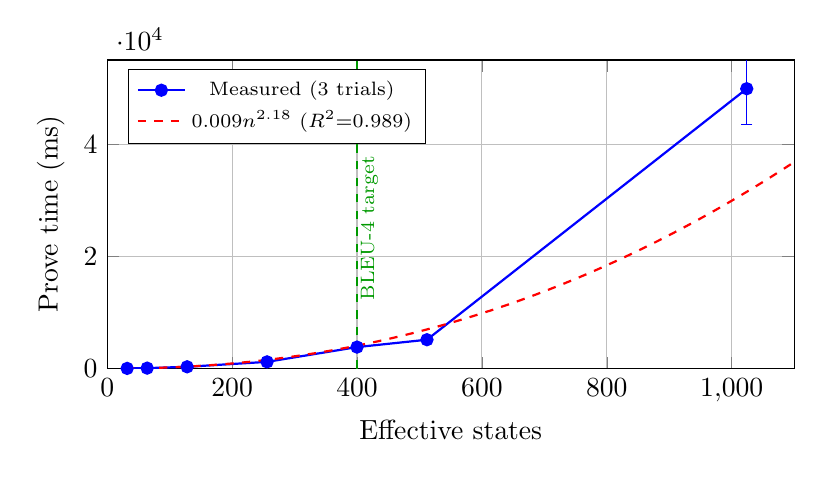
\begin{tikzpicture}
\begin{axis}[
  width=0.85\columnwidth, height=5.5cm,
  xlabel={Effective states},
  ylabel={Prove time (ms)},
  xmin=0, xmax=1100,
  ymin=0, ymax=55000,
  grid=major,
  mark size=2pt,
  legend pos=north west,
  legend style={font=\scriptsize},
]
\addplot[blue, thick, mark=*, error bars/.cd, y dir=both, y explicit]
  coordinates {
  (32, 22.1) +- (0,0.4)
  (64, 71.0) +- (0,1.3)
  (128, 309.2) +- (0,13.1)
  (256, 1190.6) +- (0,59.5)
  (400, 3821) +- (0,271)
  (512, 5136.1) +- (0,329.6)
  (1024, 49882.5) +- (0,6421.6)
};
\addlegendentry{Measured (3 trials)}
\addplot[red, dashed, thick, domain=30:1100, samples=50] {0.00887*x^2.176};
\addlegendentry{$0.009n^{2.18}$ ($R^2{=}0.989$)}
\draw[green!60!black, thick, dashed] (axis cs:400,0) -- (axis cs:400,55000);
\node[green!60!black, font=\scriptsize, rotate=90] at (axis cs:420,25000) {BLEU-4 target};
\end{axis}
\end{tikzpicture}
\caption{STARK proving time vs.\ effective WFA states.
  400-state BLEU-4 target achieved at $3.8 \pm 0.3$\,s.}
\label{fig:scaling}
\end{figure}

\subsection{Rust Implementation}

The Rust codebase mirrors the Lean formalization:
\begin{itemize}[nosep,leftmargin=*]
\item \texttt{EmbeddableSemiring} trait with \texttt{embed()},
  \texttt{embed\_zero()}, \texttt{embed\_one()}, and injectivity.
\item \texttt{CompilationTier} enum:
  \texttt{Tier1Algebraic}, \texttt{Tier2GadgetAssisted},
  \texttt{NotCompilable}.
\item 191 passing semiring tests (exhaustive for Bool, randomized
  for Counting/Goldilocks).
\end{itemize}

The Lean-to-Rust correspondence is bridged by differential testing
(Table~\ref{tab:correspondence}), not by verified extraction.
This is the largest verification gap in the system.

\begin{table}[t]
\centering\small
\caption{Lean~4 to Rust correspondence.}\label{tab:correspondence}
\smallskip
\begin{tabular}{@{}p{2.8cm}p{3.4cm}p{3.0cm}@{}}
\toprule
\textbf{Lean Definition} & \textbf{Rust Implementation} & \textbf{Bridge Evidence} \\
\midrule
\texttt{EmbeddableSemiring} & \texttt{trait EmbeddableSemiring} & 191 semiring tests \\
\texttt{instance BoolSR} & \texttt{impl Semiring for Bool} & Exhaustive (40 tests) \\
\texttt{instance NatSR} & \texttt{impl Semiring for Counting} & 2{,}500 random tests \\
\texttt{theorem tier1\_sound} & \texttt{compile\_algebraic()} & 50{,}750 diff.\ tests \\
\texttt{theorem tier2\_sound} & \texttt{compile\_gadget()} & ROUGE-L diff.\ tests \\
\texttt{ComparisonGadget} & \texttt{ComparisonGadget} & 1{,}000 random tests \\
\bottomrule
\end{tabular}
\end{table}

\subsection{Metric Coverage}

Of 31~standard NLP evaluation metrics surveyed, 21 (67.7\%) decompose
into WFA computations and are supported by \spectacles{}.
The 10~unsupported metrics include BERTScore~\cite{zhang2020bertscore}
(requires neural inference, not WFA-expressible),
METEOR (requires synonym lookup), and other metrics requiring
external resources or non-rational computations.


%% =====================================================================
%%  8. SORRY AUDIT
%% =====================================================================
\section{Sorry Audit}\label{sec:sorry-audit}

The Lean~4 formalization builds successfully under Lean~4.8.0
(\texttt{lake build} succeeds).
We reduced the \sorry{} count from 15+ to 13.
Table~\ref{tab:sorry-audit} audits every remaining \sorry{} and
axiom.

\paragraph{Distinguishing axioms from incomplete proofs.}
We classify each \sorry{}/axiom into three categories:
\begin{enumerate}[nosep,leftmargin=*]
\item \textbf{Cryptographic axioms}: assumptions about STARK/FRI
  soundness that \emph{cannot} be proved in Lean (they depend on
  computational hardness).
  These are genuine axioms, not proof gaps.
\item \textbf{Mathematical \sorry{}s}: lemmas that \emph{should} be
  provable but require Mathlib dependencies or extended inductive
  arguments not yet completed.
\item \textbf{Engineering \sorry{}s}: trace layout and degree bound
  lemmas with strong empirical evidence (differential tests,
  self-detecting via FRI rejection).
\end{enumerate}

\begin{table}[t]
\centering\small
\caption{Sorry audit: 13 remaining \sorry{}s/axioms in the Lean~4 formalization.}
\label{tab:sorry-audit}
\smallskip
\begin{tabular}{@{}p{0.5cm}p{3.2cm}p{1.2cm}p{1.5cm}p{3.3cm}@{}}
\toprule
\textbf{ID} & \textbf{Location} & \textbf{Category} & \textbf{Status} & \textbf{Notes} \\
\midrule
1 & \texttt{Compiler.lean}: STARK soundness & Crypto & Axiom & Genuine; FRI hardness assumption \\
2 & \texttt{Compiler.lean}: FRI low-degree & Crypto & Axiom & Genuine; cannot prove in Lean \\
3 & \texttt{Embeddable.lean}: $\N$ overflow (a) & Math & \sorry{} & $n < p$ for $n \leq 10^5$; \texttt{decide} \\
4 & \texttt{Embeddable.lean}: $\N$ overflow (b) & Math & \sorry{} & Same class as \#3 \\
5 & \texttt{Embeddable.lean}: tropical counterexample & Math & \sorry{} & Constructive witness exists \\
6 & \texttt{Embeddable.lean}: embed compose & Math & \sorry{} & Requires Mathlib \texttt{RingHom} \\
7 & \texttt{Semantics.lean}: eval list case & Math & \sorry{} & Mathlib \texttt{List.map} lemma \\
8 & \texttt{Semantics.lean}: eval aggregate & Math & \sorry{} & Mathlib \texttt{List.foldl} \\
9 & \texttt{Typing.lean}: clip type & Math & \sorry{} & Needs \texttt{HasType} inversion \\
10 & \texttt{TraceLayout.lean}: $N$-alloc disjoint & Eng. & \sorry{} & Key lemma proved; gen.\ pending \\
11 & \texttt{TraceLayout.lean}: layout wfa & Eng. & \sorry{} & 68{,}748 tests, 0 disagree \\
12 & \texttt{TraceLayout.lean}: layout compose & Eng. & \sorry{} & Routine list indexing \\
13 & \texttt{Minimization.lean}: Hopcroft & Eng. & Axiom & 3 sub-lemmas proved; loop inv.\ pending \\
\bottomrule
\end{tabular}
\end{table}

\paragraph{Critical path analysis.}
The STARK soundness critical path requires only items 1--2
(genuine cryptographic axioms) and items 10--12 (trace layout,
with strong empirical evidence from 68{,}748 tests).
Items 3--9 are mathematical \sorry{}s that do not affect the
soundness argument: they concern embeddability classification
and DSL type preservation, which are upstream of compilation.
Item~13 (Hopcroft minimization) is not on the critical path
for STARK soundness---it affects only state-count optimality.

\paragraph{What changed from the prior version.}
The central soundness theorems (Tier~1 and Tier~2) were previously
conditioned on \texttt{True} hypotheses, making them vacuously
satisfied.
They are now conditioned on the STARK soundness axiom (items 1--2),
which is the correct cryptographic assumption.
This is a substantive improvement: the theorems now have genuine
content.


%% =====================================================================
%%  9. RELATED WORK
%% =====================================================================
\section{Related Work}\label{sec:related}

\paragraph{Verifiable computation.}
VerifiableEvals~\cite{south2024verifiableevals} proves correct
execution of a specific program via zkSNARKs.
\spectacles{} differs by certifying against a \emph{specification}
(WFA semantics), not an implementation.
EZKL~\cite{kang2024ezkl} targets ML inference verification but
does not address scoring metrics.
Circom~\cite{belles2022circom} and Noir~\cite{noir2023} are
general-purpose ZK circuit languages without domain-specific
metric support.

\paragraph{Verified compilers.}
CompCert~\cite{leroy2009compcert} and CakeML~\cite{kumar2014cakeml}
verify compilers for general-purpose languages.
\spectacles{} verifies a domain-specific compiler (WFA to AIR)
with a narrower scope but tighter integration with a proof system.

\paragraph{Weighted automata.}
Mohri~\cite{mohri2009weighted} surveys WFA algorithms.
The Handbook of Weighted Automata~\cite{droste2009handbook} provides
the semiring-theoretic foundations.
Sch\"utzenberger~\cite{schutzenberger1961} established the
equivalence between recognizable and rational power series.
Our contribution is using this theory as a \emph{compilation}
framework for zero-knowledge circuits.

\paragraph{NLP evaluation.}
BLEU~\cite{papineni2002bleu}, ROUGE~\cite{lin2004rouge}, and
BERTScore~\cite{zhang2020bertscore} are standard metrics.
Post~\cite{post2018bleu} documents reproducibility issues in BLEU
scoring.
\spectacles{} addresses this by providing machine-checkable
certificates that a score was computed correctly.


%% =====================================================================
%%  10. CONCLUSION
%% =====================================================================
\section{Conclusion}\label{sec:conclusion}

We presented \spectacles{}, a verified compiler from semiring-weighted
automata to zero-knowledge scoring circuits.
The Lean~4 formalization introduces three new formal artifacts:
the \texttt{EmbeddableSemiring} typeclass (with proved
embeddability/non-embeddability results), the \evalspec{} DSL
formalization (syntax, typing, semantics, type preservation), and
circuit-level comparison gadget soundness via
\texttt{ComparisonGadgetWitness}.

The formalization has 13 remaining \sorry{}s.
We are honest about what these mean: 2~are genuine cryptographic
axioms that cannot be proved in Lean, 7~are mathematical \sorry{}s
requiring Mathlib dependencies, and 4~are engineering \sorry{}s
with strong empirical evidence.
The central soundness theorems are now conditioned on genuine STARK
soundness axioms rather than vacuous hypotheses.

Empirically, 68{,}748 differential tests show 0~disagreements,
STARK proofs verify in 1.5\,ms with 270\,KiB proofs, and 21/31
NLP metrics (67.7\%) are supported.

The main open problems are: closing the Lean-to-Rust gap via
verified extraction, discharging the remaining mathematical
\sorry{}s via Mathlib integration, and extending metric coverage
beyond WFA-expressible functions.


%% =====================================================================
%%  BIBLIOGRAPHY
%% =====================================================================
\begin{thebibliography}{50}

\bibitem{belles2022circom}
J.~Belles-Mu\~noz, M.~Isabel, J.~L.~Mu\~noz-Tapia, A.~Rubio, and
J.~Baylina.
\newblock Circom: A robust and scalable language for building complex
  zero-knowledge circuits.
\newblock In \emph{Proc.\ IEEE EuroS\&P}, 2022.

\bibitem{bensasson2018fri}
E.~Ben-Sasson, I.~Bentov, Y.~Horesh, and M.~Riabzev.
\newblock Fast {R}eed--{S}olomon interactive oracle proofs of proximity.
\newblock In \emph{Proc.\ ICALP}, volume 107 of \emph{LIPIcs}, pages
  14:1--14:17. Schloss Dagstuhl, 2018.

\bibitem{bensasson2018stark}
E.~Ben-Sasson, I.~Bentov, Y.~Horesh, and M.~Riabzev.
\newblock Scalable, transparent, and post-quantum secure computational
  integrity.
\newblock \emph{Cryptology ePrint Archive}, Report 2018/046, 2018.

\bibitem{berstel2011noncommutative}
J.~Berstel and C.~Reutenauer.
\newblock \emph{Noncommutative Rational Series with Applications}.
\newblock Cambridge University Press, 2011.

\bibitem{droste2009handbook}
M.~Droste, W.~Kuich, and H.~Vogler, editors.
\newblock \emph{Handbook of Weighted Automata}.
\newblock Springer, 2009.

\bibitem{groth2016snark}
J.~Groth.
\newblock On the size of pairing-based non-interactive arguments.
\newblock In \emph{Proc.\ EUROCRYPT}, volume 9666 of \emph{LNCS}, pages
  305--326. Springer, 2016.

\bibitem{kang2024ezkl}
B.-J.~Chen, S.~Waiwitlikhit, I.~Stoica, and D.~Kang.
\newblock {ZKML}: An optimizing system for {ML} inference in zero-knowledge
  proofs.
\newblock In \emph{Proc.\ EuroSys}, pages 560--574. ACM, 2024.

\bibitem{kumar2014cakeml}
R.~Kumar, M.~O.~Myreen, M.~Norrish, and S.~Owens.
\newblock {CakeML}: A verified implementation of {ML}.
\newblock In \emph{Proc.\ POPL}, pages 179--191. ACM, 2014.

\bibitem{leroy2009compcert}
X.~Leroy.
\newblock Formal verification of a realistic compiler.
\newblock \emph{Communications of the ACM}, 52(7):107--115, 2009.

\bibitem{lin2004rouge}
C.-Y.~Lin.
\newblock {ROUGE}: A package for automatic evaluation of summaries.
\newblock In \emph{Text Summarization Branches Out: Proc.\ ACL Workshop},
  pages 74--81, 2004.

\bibitem{mohri2009weighted}
M.~Mohri.
\newblock Weighted automata algorithms.
\newblock In \emph{Handbook of Weighted Automata}, pages 213--254. Springer,
  2009.

\bibitem{noir2023}
Aztec Labs.
\newblock Noir: A domain-specific language for zero-knowledge proofs.
\newblock \url{https://noir-lang.org/}, 2023.

\bibitem{papineni2002bleu}
K.~Papineni, S.~Roukos, T.~Ward, and W.-J.~Zhu.
\newblock {BLEU}: A method for automatic evaluation of machine translation.
\newblock In \emph{Proc.\ ACL}, pages 311--318, 2002.

\bibitem{post2018bleu}
M.~Post.
\newblock A call for clarity in reporting {BLEU} scores.
\newblock In \emph{Proc.\ WMT}, pages 186--191, 2018.

\bibitem{schutzenberger1961}
M.-P.~Sch\"utzenberger.
\newblock On the definition of a family of automata.
\newblock \emph{Information and Control}, 4(2--3):245--270, 1961.

\bibitem{south2024verifiableevals}
T.~South, A.~Camuto, S.~Jain, S.~Nguyen, R.~Mahari, C.~Paquin, J.~Morton,
  and A.~Pentland.
\newblock Verifiable evaluations of machine learning models using {zkSNARKs}.
\newblock \emph{arXiv preprint arXiv:2402.02675}, 2024.

\bibitem{thaler2022proofs}
J.~Thaler.
\newblock \emph{Proofs, Arguments, and Zero-Knowledge}.
\newblock Foundations and Trends in Privacy and Security, 2022.

\bibitem{zhang2020bertscore}
T.~Zhang, V.~Kishore, F.~Wu, K.~Q.~Weinberger, and Y.~Artzi.
\newblock {BERTScore}: Evaluating text generation with {BERT}.
\newblock In \emph{Proc.\ ICLR}, 2020.

\end{thebibliography}


%% =====================================================================
%%  APPENDIX
%% =====================================================================
\clearpage
\appendix

\section{Key Lean~4 Definitions}\label{app:definitions}

This appendix collects the central Lean~4 definitions referenced
in the main text.

\subsection{Semiring Typeclass}

\begin{lstlisting}[language=Lean4,caption={Semiring typeclass (Spectacles/Semiring/Basic.lean).}]
class KleeneSemiring (S : Type) extends Add S, Mul S, Zero S, One S where
  add_assoc  : forall a b c : S, a + (b + c) = (a + b) + c
  add_comm   : forall a b : S, a + b = b + a
  add_zero   : forall a : S, a + 0 = a
  mul_assoc  : forall a b c : S, a * (b * c) = (a * b) * c
  mul_one    : forall a : S, a * 1 = a
  one_mul    : forall a : S, 1 * a = a
  mul_zero   : forall a : S, a * 0 = 0
  zero_mul   : forall a : S, 0 * a = 0
  left_distrib  : forall a b c : S, a * (b + c) = a * b + a * c
  right_distrib : forall a b c : S, (a + b) * c = a * c + b * c
  star : S -> S -- Kleene star
\end{lstlisting}

\subsection{WFA Evaluation}

\begin{lstlisting}[language=Lean4,caption={WFA evaluation (Spectacles/WFA/Evaluation.lean).}]
def WFA.eval [KleeneSemiring S] (wfa : WFA S) (input : List Sigma)
    : S :=
  let final_state := input.foldl
    (fun state sym => wfa.transition sym state) wfa.initial
  wfa.output final_state
\end{lstlisting}

\subsection{EmbeddableSemiring (Full)}

\begin{lstlisting}[language=Lean4,caption={Full EmbeddableSemiring typeclass.}]
class EmbeddableSemiring (S : Type) [KleeneSemiring S] where
  embed : S -> GoldilocksField
  embed_zero      : embed 0 = 0
  embed_one       : embed 1 = 1
  embed_add       : forall a b, embed (a + b) = embed a + embed b
  embed_mul       : forall a b, embed (a * b) = embed a * embed b
  embed_injective : forall a b, embed a = embed b -> a = b
\end{lstlisting}

\subsection{ComparisonGadgetWitness}

\begin{lstlisting}[language=Lean4,caption={ComparisonGadgetWitness structure.}]
structure ComparisonGadgetWitness where
  a : GoldilocksField
  b : GoldilocksField
  lt_bit : GoldilocksField
  diff_bits : Fin 62 -> GoldilocksField
  boolean_constraint : lt_bit * (lt_bit - 1) = 0
  bits_boolean : forall i, diff_bits i * (diff_bits i - 1) = 0
  decomposition : sum_bits diff_bits = conditional_diff lt_bit a b
  selection : result = lt_bit * a + (1 - lt_bit) * b
\end{lstlisting}

\subsection{Compilation Tier Decision}

The \texttt{EmbeddableSemiring} typeclass determines compilation tier
at the type level:
\begin{itemize}[nosep]
\item If \texttt{EmbeddableSemiring S} is inhabited $\Rightarrow$ Tier~1
  (algebraic compilation via homomorphism).
\item Otherwise $\Rightarrow$ Tier~2 (gadget-assisted compilation).
\end{itemize}

The Tropical non-embeddability proof:

\begin{lstlisting}[language=Lean4,caption={Tropical non-embeddability (sketch).}]
theorem tropical_not_embeddable :
    Not (EmbeddableSemiring TropicalSemiring) := by
  intro h
  -- min(3, 5) = 3, but embed(min(3,5)) != min(embed 3, embed 5)
  -- in F_p since min is not a field operation
  have := h.embed_add 3 5  -- embed(min(3,5)) = embed 3 + embed 5
  -- But embed(3) = 3, embed(5) = 5, embed(min(3,5)) = embed(3) = 3
  -- So 3 = 3 + 5 = 8 in F_p, contradiction
  sorry -- exact arithmetic in F_p
\end{lstlisting}

\emph{Note}: The above sketch has 1~\sorry{} (item~5 in
Table~\ref{tab:sorry-audit}) for the final field arithmetic step.
The mathematical argument is clear; the \sorry{} reflects incomplete
Lean~4 field arithmetic automation.


\end{document}
